\documentclass[8pt]{article}
\usepackage[utf8]{inputenc}
\usepackage{color, hyperref, amsmath, graphicx} %, Rd}
\usepackage{framed}
\usepackage{alltt}

\setlength{\oddsidemargin}{0in}
\setlength{\topmargin}{0in}
\setlength{\textwidth}{6.5in} \setlength{\textheight}{8.5in}

%% maxwidth is the original width if it is less than linewidth
%% otherwise use linewidth (to make sure the graphics do not exceed the margin)
\makeatletter
\def\maxwidth{ %
	\ifdim\Gin@nat@width>\linewidth
	\linewidth
	\else
	\Gin@nat@width
	\fi
}
\makeatother

\definecolor{fgcolor}{rgb}{0.345, 0.345, 0.345}
\newcommand{\hlnum}[1]{\textcolor[rgb]{0.686,0.059,0.569}{#1}}%
\newcommand{\hlstr}[1]{\textcolor[rgb]{0.192,0.494,0.8}{#1}}%
\newcommand{\hlcom}[1]{\textcolor[rgb]{0.678,0.584,0.686}{\textit{#1}}}%
\newcommand{\hlopt}[1]{\textcolor[rgb]{0,0,0}{#1}}%
\newcommand{\hlstd}[1]{\textcolor[rgb]{0.345,0.345,0.345}{#1}}%
\newcommand{\hlkwa}[1]{\textcolor[rgb]{0.161,0.373,0.58}{\textbf{#1}}}%
\newcommand{\hlkwb}[1]{\textcolor[rgb]{0.69,0.353,0.396}{#1}}%
\newcommand{\hlkwc}[1]{\textcolor[rgb]{0.333,0.667,0.333}{#1}}%
\newcommand{\hlkwd}[1]{\textcolor[rgb]{0.737,0.353,0.396}{\textbf{#1}}}%

\usepackage{framed}
\makeatletter
\newenvironment{kframe}{%
	\def\at@end@of@kframe{}%
	\ifinner\ifhmode%
	\def\at@end@of@kframe{\end{minipage}}%
\begin{minipage}{\columnwidth}%
	\fi\fi%
	\def\FrameCommand##1{\hskip\@totalleftmargin \hskip-\fboxsep
		\colorbox{shadecolor}{##1}\hskip-\fboxsep
		% There is no \\@totalrightmargin, so:
		\hskip-\linewidth \hskip-\@totalleftmargin \hskip\columnwidth}%
	\MakeFramed {\advance\hsize-\width
		\@totalleftmargin\z@ \linewidth\hsize
		\@setminipage}}%
{\par\unskip\endMakeFramed%
	\at@end@of@kframe}
\makeatother

\definecolor{shadecolor}{rgb}{.97, .97, .97}
\definecolor{messagecolor}{rgb}{0, 0, 0}
\definecolor{warningcolor}{rgb}{1, 0, 1}
\definecolor{errorcolor}{rgb}{1, 0, 0}
\newenvironment{knitrout}{}{} % an empty environment to be redefined in TeX

% set up headers and footers
\usepackage{fancyhdr}
\pagestyle{fancy}
\lhead{PH 290: Project 1}
\chead{}
\rhead{Jin Rou New}
\lfoot{}
\cfoot{}
\rfoot{\thepage}

%% for inline R code: if the inline code is not correctly parsed, you will see a message
\newcommand{\rinline}[1]{SOMETHING WRONG WITH knitr}

\usepackage{titling}
\setlength{\droptitle}{-10em} % Remove spacing before title

\usepackage{titlesec}
\titlespacing{\section}{0pt}{\parskip}{-\parskip}
%\titlespacing{\subsection}{0pt}{\parskip}{-\parskip}
%\titlespacing{\subsubsection}{0pt}{\parskip}{-\parskip}

\title{PH290: Kaggle Heritage Health Prize Competition Project}
\author{Jin Rou New\\
	SID: 25944841
%	\\ University of California, Berkeley
	}

\date{\vspace{-5ex}} % Remove date to save space
%\date{\today}

\setlength\parindent{0pt}
\setlength{\parskip}{\baselineskip} % to get space between paragraphs
\usepackage{setspace} % to allow for double line spacing
\begin{document}
\maketitle
%\renewcommand{\abstractname}{}
%==================================================
%Data analysis: (a) summarize the winning methods; (b) propose your own
%solution and do a comparison; (c) carry out an analysis to address your
%own question.
%
%The report is no more than 3 pages, including tables and figures (and
%references, everything).
%{ At the beginning of the report, prepare a summary of your findings (what
%kind of useful knowledge you have obtained via your analysis).
%{ Make sure to include a description on how you process the data.
%==================================================
\section{Summary}
\label{sec:summary}
The most important predictors of the number of days a patient will spend in hospital in the following year are: the patient's sex and age at first claim, total number of claims in the current year, number of pregnancy-related claims, hospital inpatient claims and emergency-related claims in the current year, pay delay of claim in the current year, number of unique health providers among the patient's claims in the current year. Both Random Forest (RF) and a Gradient Boosting Machine (GBM) were used to fit the model and the latter gives marginally better performance. My analysis also showed that the most important predictors of pay delay on claims are: Procedure Group (Pathology and Lab, Evaluation and Management, Surgery (genital system and integumentary system)), Specialty (Surgery, Diagnostic Imaging, Radiology), Primary Condition (Other renal diseases, Cancer B) and Place of Service (Office).
%==================================================
\section{Introduction}
\label{sec:introduction}
The Heritage Health Prize Competition is a Kaggle competition in which the goal is to create an algorithm that predicts how many days a patient will spend in the hospital in Year 4, given previous years' claim data from members of the Heritage Provider Network. The accuracy of the algorithm is evaluated based on the root mean log squared error (RMLSE). In this paper, instead of predicting the number of days in hospital in Year 4 given data from Years 1-3, I will predict the number of days in hospital in Year 3 given data from Years 1-2. This is because the competition is closed to submissions and Year 4 data is not released so it is no longer possible to calculate the RMLSE for Year 4.
%==================================================
\section{Data processing and feature engineering} 
\label{sec:data-processing}
The data is organized into a relational database with separate tables on member data, claims data, lab test data, prescription data and days in hospital data. The first step is to join all the tables into one and aggregating the data such that each row corresponds to a member instead of a claim. Categorical variables with ordinal values were converted to numeric ones (e.g. age 0-9 to 5). Missing values for quantitative variables were inputed by the mean of that variable for that year.

This data processing step occurs concomitantly with the feature engineering step, in which the available member-level information is summarized in a variety of ways, e.g. information from the drugs table by year were summarized into the following variables by year: total number of drug claims, total/mean/minimum/ maximum/range of/standard deviation of/last drug count, claim-level vendor info was aggregated into number of unique vendors per member per year, claim-level Primary Condition Group (PCG) info for each was condensed into number of claims for each PCG per member per year. This resulted in a total of 143 member-level features for 76038 members in Year 1 in the training set and 71435 members in Year 2 in the test set.
%==================================================
\section{Proposed method}
I applied both a Random Forest (RF) and a Gradient Boosting Machine (GBM) to the processed data set. Relative importance of the top 20 most important predictors of both models are given in Figure~\ref{fig:importance}. The following predictors belong in the top 20 most important predictors for both models: Sex, PrimaryConditionGroupPRGNCYCount, PayDelayMean, AgeAtFirstClaimNum, PayDelayTotal, PlaceSvcInpatientHospitalCount, ClaimCount, ProviderIDCount, SpecialtyEmergencyCount. Most of these make sense, although it is odd that PayDelay would be an important predictor; though this could be related to some underlying confounder.

\begin{figure}[htb]
	\begin{center}
		\begin{tabular}{|c|c|}\hline 
			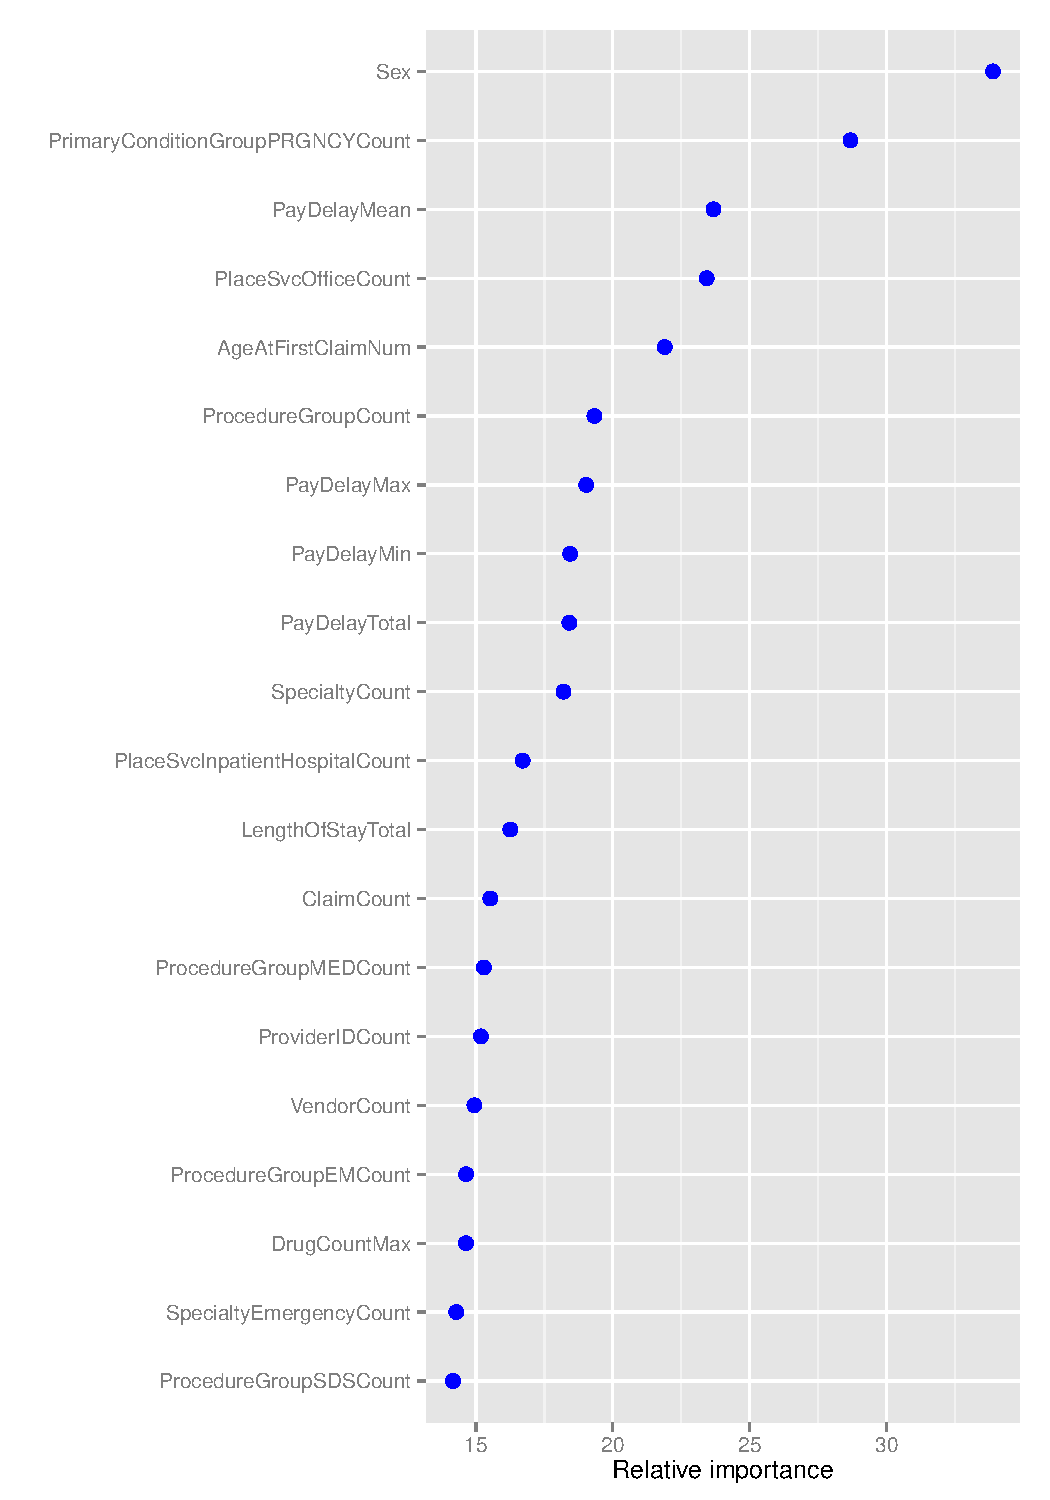
\includegraphics[width = 0.4\textwidth]{results/rf-importance.pdf} & 
			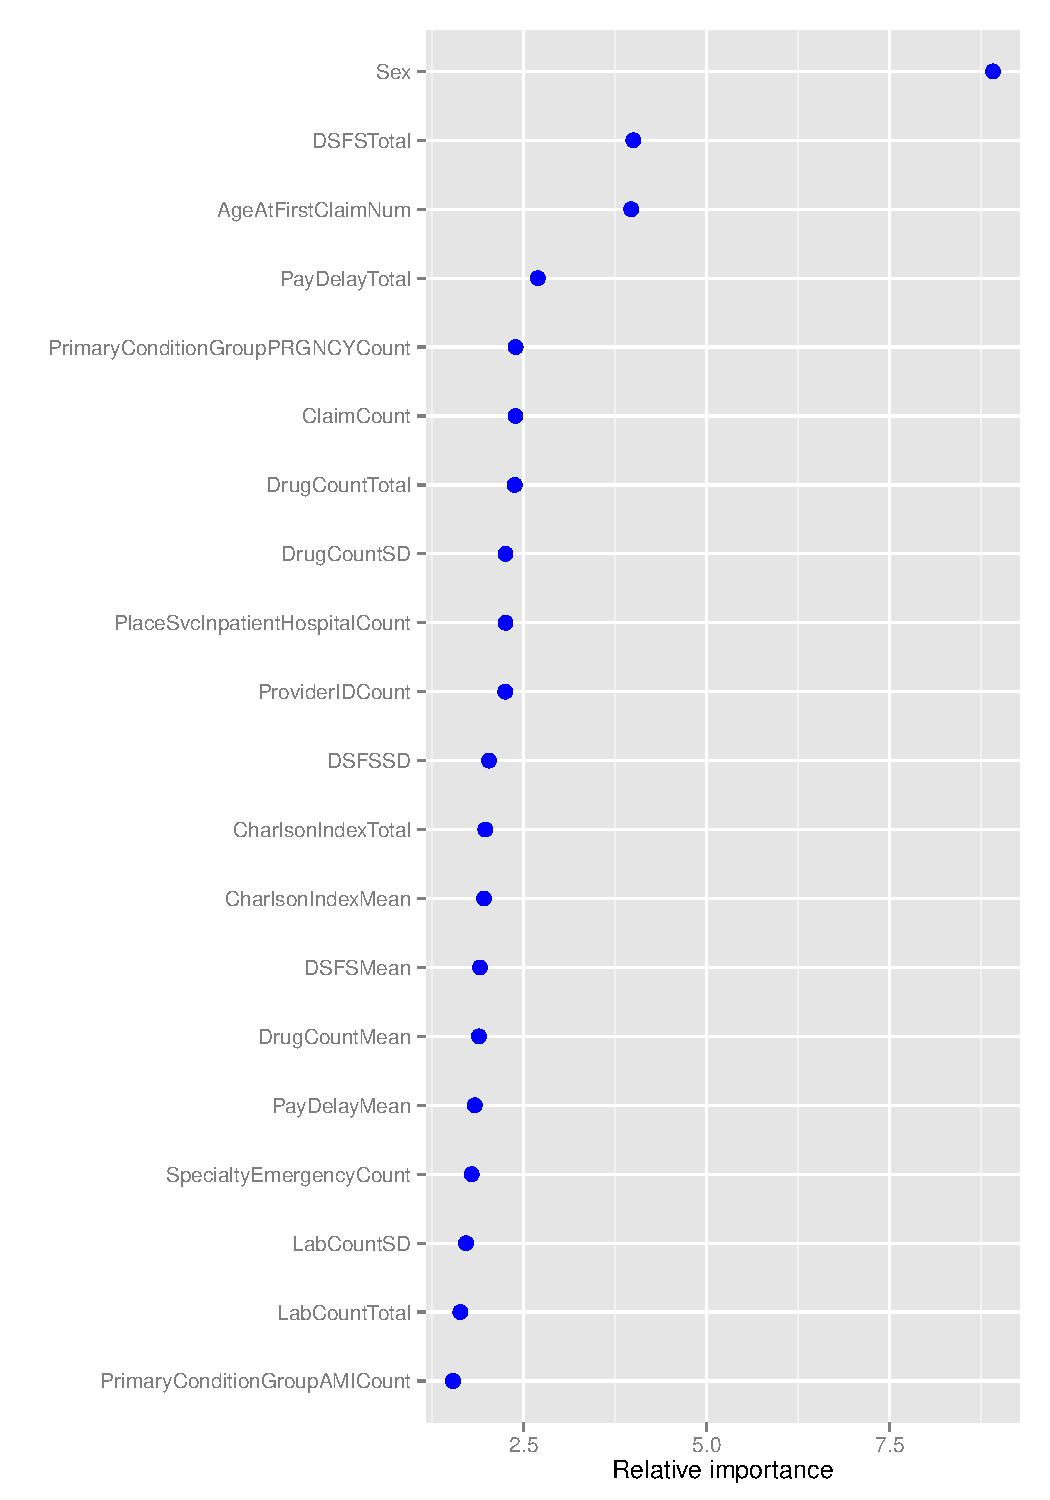
\includegraphics[width = 0.4\textwidth]{results/gbm-importance.pdf} \\ \hline
		\end{tabular}
		\caption{{\bf Variables ranked by variable relative importance for the models Random Forest (left) and Gradient Boosting Machine.}}
		\label{fig:importance}
	\end{center}
\end{figure}

%All calculations were carried out in the R programming language, with additional functions from the \texttt{tidyr} and \texttt{dplyr} packages for data processing and from the \texttt{randomForest} and \texttt{gbm} packages for modelling. 
%==================================================
\section{Method benchmarking}
\label{sec:comparison}
All winning methods employed a combination of many different models.
Models are combined by blending and the final predictions are linear combinations of the predictions of all models in the blend, with weights given based on a ridge regression performed on the leaderboard scores (e.g. [1-3]). The base models that make up the final combination include: Stochastic Gradient Descent Models [1-3], Gradient Boosting Machines [2-5], Neural Networks [4-5], Linear Models [4-5], Tree Ensemble [2-3], Random Forests [4-6], Additive Groves [5], Multivariate Adaptive Regression Splines [5], Regularized Greedy Forests [6], Gradient Boosting Decision Trees [6] and optimized constant value models [2-5].

A fair comparison between my method and the winning methods was not possible given that the winning methods used all available data to predict the days in hospital for Year 4 while I used data up to Year 2 to predict the days in hospital for Year 3. Moreover, I was unable to reproduce exactly the winning methods to check their performance with Year 2 data on Year 3 predictions.

Instead, we can compare my methods against the base models of 1) setting the prediction to 0 days for all patients 2) setting the prediction to the mean of days in hospital in Year 2 for all patients. The first model gives an RMLSE of 0.4262385 while the second gives a RMLSE of 0.3871215. In comparison, the RF results in a RMLSE of 0.3771039 while GBM gives 0.3765514.
%==================================================
\section{Additional analyses}
\label{sec:addition}
I was interested in the pay delay on claims. The mean pay delay is about 43 days (assuming no pay delay more than 162 days), which should be possible to optimize for greater operational efficiency and member satisfaction. Applying a GBM on claim-level data and looking at variable relative importance, I found that the 10 most important predictors of pay delay are (as shown in Figure~\ref{fig:importance-paydelay}): ProcedureGroupPL, ProcedureGroupEM, SpecialtySurgery, PrimaryConditionGroupRENAL3, SpecialtyDiagnosticImaging, ProcedureGroupRAD, PrimaryConditionGroupCANCRB, PlaceSvcOffice, ProcedureGroupSGS and ProcedureGroupSIS.

\begin{figure}[htbp]
	\begin{center}
		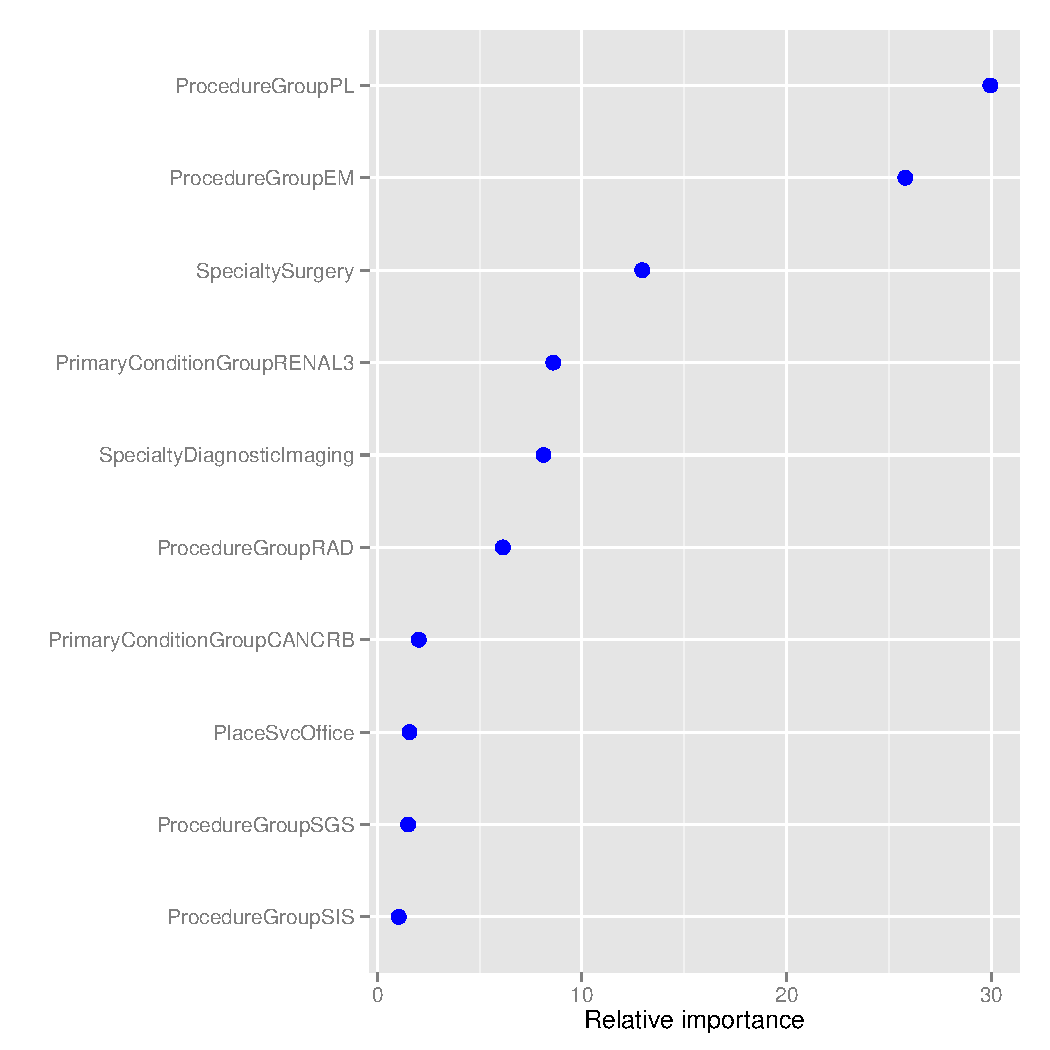
\includegraphics[width = 0.4\textwidth]{results/gbm-paydelay-importance.pdf}
		\caption{{\bf Variables ranked by variable relative importance for the Gradient Boosting Machine on claim-level pay delay data.}}
		\label{fig:importance-paydelay}
	\end{center}
\end{figure}

%==================================================
\section{Discussion} 
\label{sec:discussion}
While the RF and GBM perform better than the base models, there is likely still room for improvement, such as parameter tuning using cross-validation. More models such as Generalized Linear Models, Neural Nets etc. can be fitted and a mix of the models can be blended to yield a lower RMLSE.
%==================================================
\section{References}
{\tiny
1. Mestrom, W. (2011). My milestone 1 solution to the Heritage Health Prize. \\
2. de Grijs, E. and Mestrom, W. (2012a). Our milestone 2 solution of the Heritage Health Prize.\\
3. de Grijs, E. and Mestrom, W. (2012b). Our milestone 3 solution of the Heritage Health Prize.\\
4. Brierley, P., Vogel, D. and Axelrod, R. (2011). Heritage Provider Network Health Prize Round 1 Milestone Prize: How We Did It – Team `Market Makers'\\
5. Brierley, P., Vogel, D. and Axelrod, R. (2012). Heritage Provider Network Health Prize Round 2 Milestone Prize: How We Did It – Team `Market Makers'\\
6. Johnson, R. and Zhang, T. (2012). Heritage Provider Network Health Prize Round 3 Milestone: Team crescendo’s Solution.
}
\end{document}
